\documentclass[preview]{standalone}

\usepackage{amsmath}
\usepackage{amssymb}
\usepackage{stellar}
\usepackage{bettelini}
\usepackage{wrapfig}

\hypersetup{
    colorlinks=true,
    linkcolor=black,
    urlcolor=blue,
    pdftitle={Biologia},
    pdfpagemode=FullScreen,
}

\begin{document}

\id{biologia-produzione-proteine}
\genpage

\section{Produzione di proteine}

\begin{snippet}{820921be-f4a8-4466-8a2a-1f36c7064ac6}
    Le proteine vengono prodotte con le informazioni (nel nucleo).
    Quando l'informazione è necessaria ne viene fatta una copia nel nucleo.
    Questa informazione viene letta dal ribosoma.
    Il ribosoma legge l'mRNA,
    dove c'è scritto dove mettere gli amminoacidi per costruire le proteine.
\end{snippet}

\begin{snippet}{prod-cellula-2-illustration}
    \setlength{\intextsep}{0pt}%
    \begin{wrapfigure}{l}{0.525\textwidth}
        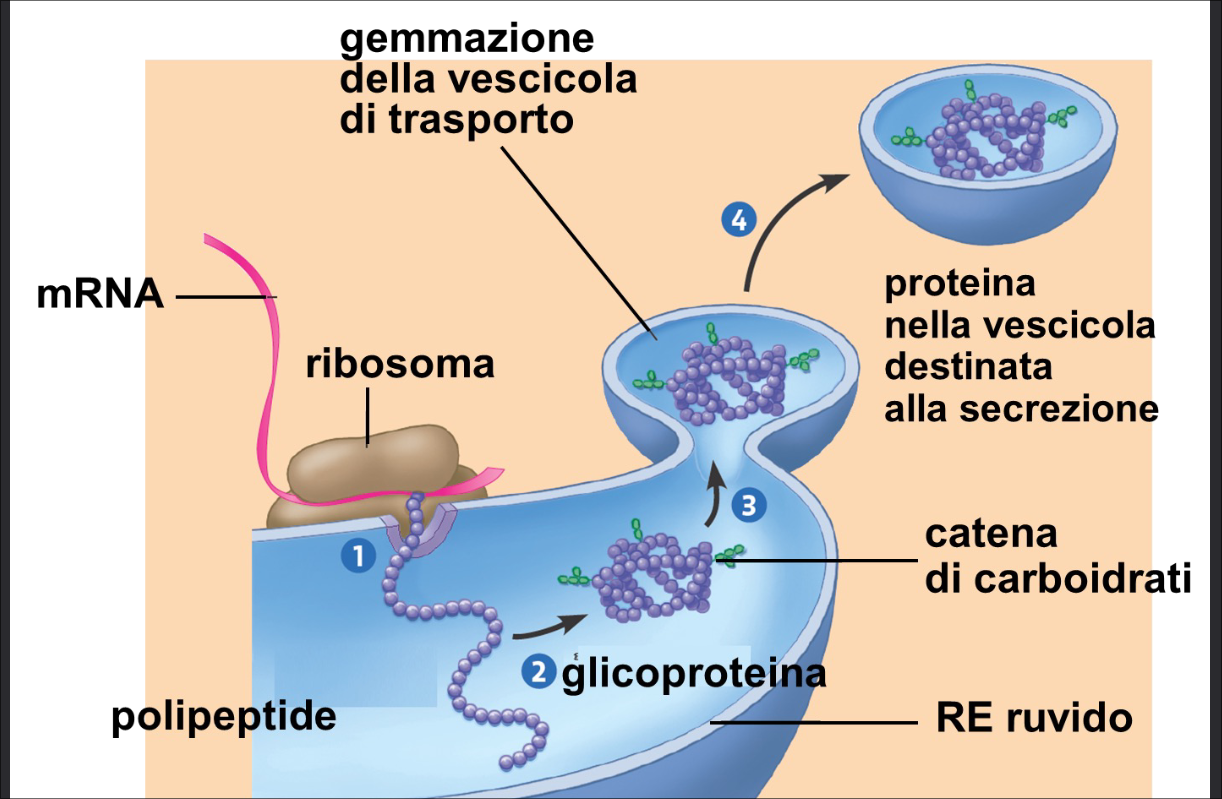
\includegraphics[width=0.5\textwidth]{./resources/prod-cellula2.png}
    \end{wrapfigure}

    % che sia una glicoproteina è un esempio
    Il contorno blu rappresenta il reticolo endoplasmatico.
    Il ribosoma si appoggia su di essa ed inserisce la proteina.
    La vescicola del reticolo si stacca e si unisce all'apparato di Goigi, dove le proteine
    vengono completate e indirizzate.
    La proteina se ne va nuovamente con una vescicola, la vescicola si fonde alla membrana (diventa parte della membrana)
    e per esocitosi ne uscirà il contenuto.

    \wrapfill
\end{snippet}

\begin{snippet}{prod-cellula-illustration}
    \setlength{\intextsep}{0pt}%
    \begin{wrapfigure}{l}{0.7\textwidth}
        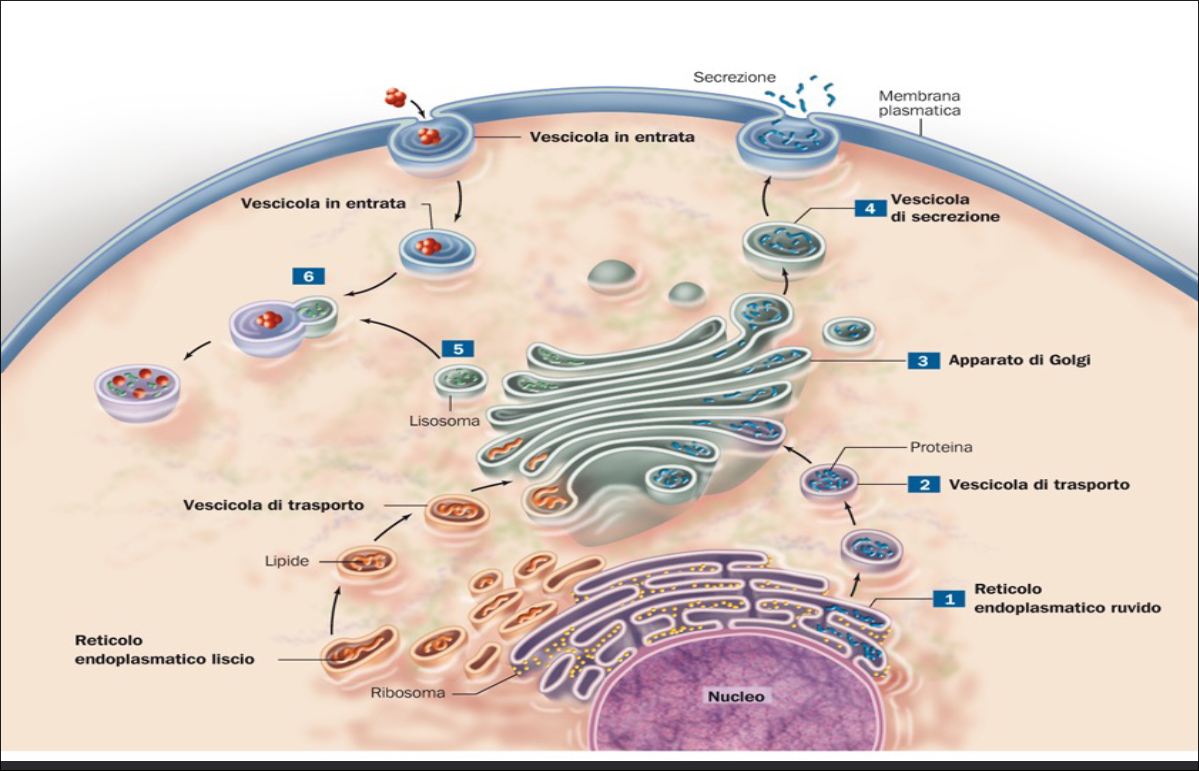
\includegraphics[width=0.7\textwidth]{./resources/prod_cellula.png}
        \caption{Produzione proteina 2}
        \vspace{-1cm}
    \end{wrapfigure}
    
    Nel reticolo endoplasmatico liscio vengono creati dei fosfolipidi.
    Siccome le vescicole accorciano il reticolo, questi fosfolipidi servono a ricaricarlo.
    
    Gli enzimi dei lisosomi vengono costruiti dai ribosomi nel reticolo endoplasmatico ruvido.
    
    \wrapfill
\end{snippet}

\begin{snippet}{categorie-cellule-termini}
    La seguente lista associa categorie ad alcuni termini:
    \begin{itemize}
        \item \textbf{Controllo dell'informazione genetica:}
            nucleo, ribosoma.
        \item \textbf{Poduzione di energia:}
            mitocondrio, cloroplasti.
        \item \textbf{Costruzione, distribuzione e degradazione:}
            reticolo endoplasmatico ruvido,
            reticolo endoplasmatico liscio, apparato di Golgi,
            lisosomi, vacuoli, perossisomi, ribosomi.
        \item \textbf{Supporto fisico, movimento e comunicazione tra le cellule:}
            citoscheletro, membrana plasmatica, matrice extracellulare,
            giunzione cellulare, parete cellulare, flagelli.
    \end{itemize}
\end{snippet}

\end{document}